\begin{figure}
    \centering
    \captionsetup[subfigure]{labelformat=empty}
\begin{subfigure}{.5\textwidth}
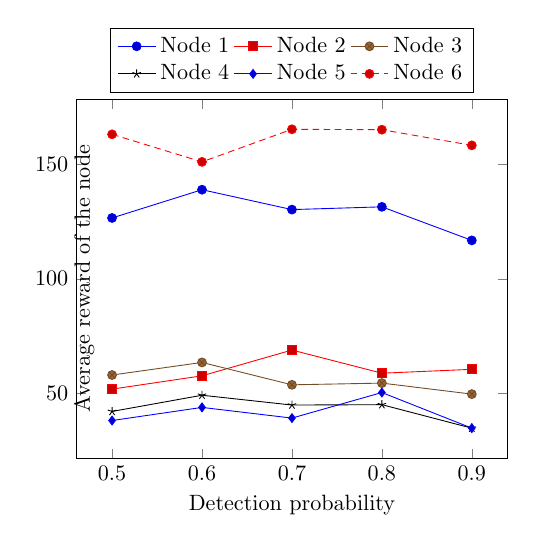
\begin{tikzpicture}[scale=0.8]
\begin{axis}[
  xlabel={Detection probability},
  ylabel={Average reward of the node },
  y label style={at={(0.06,0.5)}},
  xtick={0.5,0.6,0.7,0.8,0.9,1.0},
  legend style={at={(0.5,1.2)},cells={align=right}, anchor=north,legend columns=3},
  grid style=dashed,
]

\addplot+[]
    coordinates {
(0.5,126.469294224)(0.6,138.768688772)(0.7,130.10979383)(0.8,131.308647284)(0.9,116.70873472)
};

\addplot+[]
    coordinates {
(0.5,51.9774584454)(0.6,57.7615872131)(0.7,68.9811633084)(0.8,58.9060250618)(0.9,60.5911805552)
};

\addplot+[]
    coordinates {
(0.5,58.112876005)(0.6,63.5894390224)(0.7,53.8483204974)(0.8,54.5969922461)(0.9,49.8027670671)
};

\addplot+[]
    coordinates {
(0.5,42.2594496478)(0.6,49.3133895991)(0.7,45.0502147208)(0.8,45.20918204)(0.9,34.9808016775)
};

\addplot+[]
    coordinates {
(0.5,38.3055097066)(0.6,44.0188235767)(0.7,39.3680288222)(0.8,50.4912779668)(0.9,34.9978557067)
};

\addplot+[]
    coordinates {
(0.5,162.87848727)(0.6,150.876767477)(0.7,165.06110317)(0.8,164.882126918)(0.9,158.067481047)
};

\legend{Node 1, Node 2, Node 3, Node 4, Node 5, Node 6}
\end{axis}
\end{tikzpicture}

\caption{Scenario c)}
\label{fig:nodeimp_topofullmesh_single}
\end{subfigure}
\begin{subfigure}{.33\textwidth}
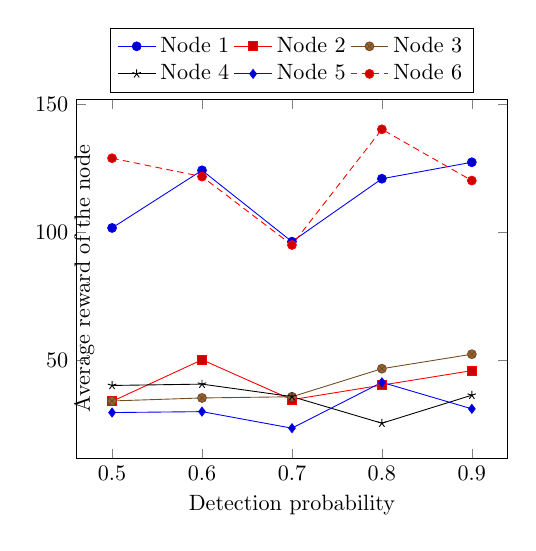
\begin{tikzpicture}[scale=0.8]
\begin{axis}[
  xlabel={Detection probability},
  ylabel={Average reward of the node },
  y label style={at={(0.06,0.5)}},
  xtick={0.5,0.6,0.7,0.8,0.9,1.0},
  legend style={at={(0.5,1.2)},cells={align=right}, anchor=north,legend columns=3},
  grid style=dashed,
]
\addplot+[]
    coordinates {
(0.5,101.616873023)(0.6,124.145242333)(0.7,96.2616914651)(0.8,120.862819291)(0.9,127.305784272)
};

\addplot+[]
    coordinates {
(0.5,33.8037034841)(0.6,50.0693289402)(0.7,34.460597311)(0.8,40.1535742549)(0.9,45.8166364524)
};

\addplot+[]
    coordinates {
(0.5,33.9581528218)(0.6,35.1326808601)(0.7,35.6074089582)(0.8,46.5769811834)(0.9,52.2400544067)
};

\addplot+[]
    coordinates {
(0.5,40.0224063598)(0.6,40.5434953331)(0.7,35.6681036149)(0.8,25.2556265302)(0.9,36.2111392677)
};

\addplot+[]
    coordinates {
(0.5,29.4251886633)(0.6,29.7859232959)(0.7,23.3183642626)(0.8,41.2471235042)(0.9,30.8838558151)
};

\addplot+[]
    coordinates {
(0.5,128.882560148)(0.6,121.704109507)(0.7,94.9489538016)(0.8,140.19719198)(0.9,120.142225907)
};


\legend{Node 1, Node 2, Node 3, Node 4, Node 5, Node 6}
\end{axis}
\end{tikzpicture}

\caption{Scenario d)}
\label{fig:nodeimp_topofullmesh_multiple}
\end{subfigure}
\caption{Results for single and multiple attackers}
    \label{fig:mdp-result-fullmesh}
\end{figure}